\documentclass[a4paper, 12pt]{article}

% Подключение русского языка.
\usepackage[russian]{babel}
\usepackage[utf8]{inputenc}
\usepackage[T2A]{fontenc}

% Настройка внешнего вида заголовков.
\usepackage{titlesec}
\newcommand{\chapterFont}{\fontsize{16}{15} \selectfont}
\newcommand{\chapterNumberFont}{\fontsize{14}{15} \selectfont}
\newcommand{\sectionFont}{\fontsize{14}{15} \selectfont}
\renewcommand\thesection{\thechapter.\arabic{section}.}
\titleformat{\chapter}[display]
{\normalfont \chapterFont \bfseries}{\centering \chapterNumberFont
	\chaptertitlename \ \thechapter}{10pt}{\centering \chapterFont}
\titlespacing{\chapter}{0pt}{8pt}{25pt}
\titleformat{\section}
{\normalfont \sectionFont \bfseries}{\centering \thesection}{6pt}
{\centering \sectionFont}
\titlespacing{\section}{0pt}{25pt}{5pt}
% Настройка размеров страниц.
\setlength{\parindent}{0pt} \renewcommand{\baselinestretch}{1.2} \topmargin = 0mm \textwidth =
175mm \textheight = 260mm \hoffset = -17.5mm \voffset = -25.5mm
% Подключение библиотек для изображений.
\usepackage{tcolorbox}
\usepackage{graphicx}
\usepackage{float}
% Подключение библиотек для математических символов.
\usepackage{amsthm}
\usepackage{parcolumns}
\usepackage{amsmath}
\usepackage{amsfonts}
% Настройка внешнего вида для теорем, утверждений и т.д.
\theoremstyle{definition}
\newtheorem*{theorem}{Теорема}
\newtheorem*{definition}{Определение}
\newtheorem*{example}{Пример}
\newtheorem*{remark}{Замечание}
\newtheorem*{solution}{Решение}

\begin{document}

\section*{Задача 1104}
Найти общее решение дифференциального уравнения:
$$(1 - x)y'' - 2y' + y = 0$$

\begin{solution}
   Решим задачу методом рядов.

   1) Предположим, что решение имеет вид:
   $$y = \sum_{k = 0}^{\infty} y_k x^k$$

   2) Тогда:
   $$y' = \sum_{k = 0}^{\infty} y_k k x^{k-1}$$
   $$y'' = \sum_{k = 0}^{\infty} y_k k(k-1) x^{k-2}$$

   3) Подставляем в исходное уравнение:
   $$\sum_{k = 0}^{\infty} y_k k(k-1)x^{k-2} - y_k k(k-1)x^{k-1} - 2y_k kx^{k-1} + y_k x^k = 0$$

   4) Приравнивая коэффициенты при $x^k$:
   $$y_k - k(k+1)y_{k+1} - 2(k+1)y_{k+1} + y_{k+2}(k+1)(k+2) = 0$$

   5) Рекуррентное соотношение:
   $$y_{k+2} = \frac{y_{k+1}(k+1)(k+2) - y_k}{(k+1)(k+2)}$$

   6) Два линейно независимых решения:

   Первое решение ($y_0 = 1, y_1 = 0$):
   $$y_1 = 1 - \frac{1}{2}x - \frac{1}{2}x^2 - \frac{11}{24}x^3 + \cdots$$

   Второе решение ($y_0 = 0, y_1 = 1$):
   $$y_2 = x + \frac{5}{6}x^2 + \frac{3}{4}x^3 + \cdots$$

   Таким образом, общее решение:
   $$y = c_1y_1 + c_2y_2$$
   где $c_1$ и $c_2$ — произвольные константы.
\end{solution}
\section*{Задача 1106}
Найти общее решение дифференциального уравнения:
$$y'' - xy' + xy = 0$$

\begin{solution}
1) Предположим решение в виде степенного ряда:
   $$y = \sum_{k = 0}^{\infty} y_k x^k$$

2) Производные:
   $$y' = \sum_{k = 0}^{\infty} y_k k x^{k-1}$$
   $$y'' = \sum_{k = 0}^{\infty} y_k k(k-1) x^{k-2}$$

3) Подставляем и приравниваем коэффициенты:
   $$y_{k+3} = \frac{y_{k+1}(k+1) - y_k}{(k+3)(k+2)}$$

4) Три линейно независимых решения:

   Первое решение ($y_0 = 1, y_1 = 0, y_2 = 0$):
   $$y_1 = 1 - \frac{1}{6}x^3 - \frac{1}{40}x^5 + \cdots$$

   Второе решение ($y_0 = 0, y_1 = 1, y_2 = 0$):
   $$y_2 = x + \frac{1}{6}x^3 - \frac{1}{12}x^4 + \frac{1}{40}x^5 + \cdots$$

   Третье решение ($y_0 = 0, y_1 = 0, y_2 = 1$):
   $$y_3 = x^2 + \frac{1}{6}x^4 - \frac{1}{40}x^5 + \cdots$$

Таким образом, общее решение:
$$y = c_1y_1 + c_2y_2 + c_3y_3$$
где $c_1$, $c_2$ и $c_3$ — произвольные константы.
\end{solution}

\section*{Задача 1110}
Найти общее решение дифференциального уравнения:
$$ xy'' + 2y' + xy = 0 $$
\begin{solution}
    1) При $x_0 = 0 $ : $ p_0(0) = 0 $ => $ \sum_{k = 0}^{\infty} y_k x^{k + \alpha} $ \par
    2) Преобразуем: $$ \sum_{k = 0}^{\infty} y_k (k + \alpha) (k + \alpha - 1) x^{k + \alpha - 2 + 1} + 2 \sum_{k = 0}^{\infty} y_k (k + \alpha) x^{k + \alpha - 1} + \sum_{k = 0}^{\infty} y_k x^{k + \alpha + 1} = 0 $$
    3) min степень $x$: $ k + \alpha - 1 $, $ k = 0 $ => $ \alpha - 1 $ => \par
    при $ k = 0 $: $ y_0 \alpha (\alpha - 1) x^{\alpha - 1} + 2 y_0 \alpha x^{\alpha - 1} + y_0 x^{\alpha + 1} $ \par
    $ y_0 (\alpha (\alpha - 1) + 2 \alpha) $, где $ (\alpha (\alpha - 1) + 2 \alpha) = 0 $, при $ x^{\alpha - 1} $ (минимальная степень $x$) \par
    $ \alpha (\alpha + 1) = 0 $ => $ \alpha = 0 $; $-1$, но берем $-1$, т.к. $\alpha = 0$ делает ряд обычным. \par
    4) Получаем ряд: $$ \sum_{k = 0}^{\infty} \underset{k = p + 2}{y_k (k - 1) (k - 2) x^{k - 2}} + 2 \sum_{k = 0}^{\infty} \underset{k = p + 2}{y_k (k - 1) x^{k - 2}} + \sum_{k = 0}^{\infty} \underset{k = p}{y_k x^k = 0} $$
    5) При $ x^p $ : $$ y_{p + 2} (p + 1) + 2y_{p + 2} (p + 1) + y_p = 0 $$
    $$ y_{p + 2} (p + 1) (p + 2) + y_p = 0 $$
    $$ y_{p + 2} = -\dfrac{y_p}{(p + 1) (p + 2)} $$
    6) Построим матрицу: 
    $
        \begin{array}{ccc}
                  & 1) & 2) \\
            y_0 = & 1  & 0  \\
            y_1 = & 0  & 1  \\
        \end{array}
    $ \par
    \quad1) $ y_2 = -\dfrac{1}{2} = -\dfrac{1}{2!} $, $ y_3 = 0 $, $ y_4 = -\dfrac{-\dfrac{1}{2}}{3 \cdot 4} = \dfrac{1}{24} = \dfrac{1}{4!} $, $\cdots$ => \par
    => $ y_1 = \dfrac{1}{x} - \dfrac{x}{2!} + \dfrac{x^3}{4!} - \dfrac{x^5}{6!} + \cdots $\par
    \quad2) $ y_2 = 0 $, $ y_3 = -\dfrac{1}{1 \cdot 2 \cdot 3} = -\dfrac{1}{3!} $, $ y_4 = 0 $, $\cdots$ => \par
    => $ y_2 = 1 - \dfrac{x^2}{3!} + \dfrac{x^4}{5!} - \dfrac{x^6}{7!} + \cdots $ \par
    7) Общее решение будет выглядить так: $ y = c_1y_1 + c_2y_2 $
\end{solution}\pagebreak

\pagebreak\section*{Задача 1109}
Найти общее решение дифференциального уравнения: $$ y''' - xy'' + (x - 2)y' + y = 0 $$
\begin{solution}
    1) При $x_0 = 0 $, $ p_0(0) \neq 0 $ => $ y = \sum_{k = 0}^{\inf} y_k x^k $. \par
    2) Преобразуем: $$ \sum_{k = 0}^{\inf} \underset{k = p + 3}{k (k - 1) (k - 2) y_k x^{k - 3}} - \sum_{k = 0}^{\inf} \underset{k = p + 1}{k (k - 1) y_k x^{k -2 + 1}} + \sum_{k = 0}^{\inf} \underset{k = p}{k y_k x^{k - 1 + 1}} - 2 \sum_{k = 0}^{\inf} \underset{k = p + 1}{k y_k x^{k - 1}} + \sum_{k = 0}^{\inf} \underset{k = p}{y_k x^k} = 0 $$
    При $ x^p $ : $$ (p + 3) (p + 2) (p + 1) y_{p + 3} - (p + 1) p y_{p + 1} + p y_p - 2 (p + 1) + y_p = 0 $$
    Сократим $ (p + 1) $ : $$ (p + 3) (p + 2) y_{p + 3} - (p + 2) y_{p + 1} + y_p = 0 $$
    3) Выразим $ y $ : $$ y_{p + 3} = \frac{y_{p + 1}}{p + 3} - \frac{y_p}{(p + 3)(p + 2)} $$
    4) Построим единичную матрицу: \par
    $$\begin{array}{c ccc}
                      & 1) & 2) & 3) \\
                y_0 = & 1  & 0  & 0  \\
                y_1 = & 0  & 1  & 0  \\
                y_2 = & 0  & 0  & 1  \\
            \end{array}$$\par
    \quad1) $ y_3 = 0 - \frac{1}{6} = -\frac{1}{6} $, $ y_4 = 0 $, $ y_1 = 1 - \frac{x^3}{6} + 0 + \cdots $\par
    \quad2) $ y_3 = \frac{1}{3} - 0 = \frac{1}{3} $, $ y_4 = -\frac{1}{12} $, $ y_2 = x + \frac{x^3}{3} - \frac{x^4}{12} + \cdots $\par
    \quad3) $ y_3 = 0 $, $ y_4 = \frac{1}{4} $, $ y_3 = x^2 + \frac{x^4}{4} + \cdots $\par
    5) Таким образом общее решение: $$ y = c_1y_1 + c_2y_2 + c_3y_3 $$ где $c_1$, $c_2$ и $c_3$ - произвольные константы.

\end{solution}\pagebreak
\pagebreak\section*{Задача 1114}
Найти общее решение дифференциального уравнения: $$ x^2y'' + 2xy' - (x^2 + 2x + 2)y = 0. $$
\begin{solution}
    1) При $ x_0 = 0, p_0(0) = 0 $ => Общий случай $ y = \sum_{k = 0}^{+\infty} y_k x^{k + \alpha} $
    $$ \sum_{k = 0}^{\infty} (k + \alpha)(k + \alpha - 1) x^{k + \alpha - 2 + 2} y_k + 2 \sum_{k = 0}^{\infty} (x + \alpha) x^{k + \alpha - 1 + 1} y_k - \sum_{k = 0}^{\infty} x^{k + \alpha + 2} y_k - 2 \sum_{k = 0}^{\infty} x^{k + \alpha + 1} y_k - 2 \sum_{k = 0}^{\infty} x^{k + \alpha} y_k, $$ 
    min степень икса: $ k + \alpha, k_{min} = 0 $ => $\alpha$ \par
    2) По $ x^{\alpha}: $ $$ y_0 (\alpha (\alpha - 1) + 2\alpha - 2) $$
    $$ \alpha (\alpha - 1) + 2\alpha - 2 = 0 $$
    $$ \alpha^2 + \alpha - 2 = 0 => \alpha_1 = -2, \alpha_2 = 1. $$
    3) Рассмотрим $\alpha = 1:$
    $$ \sum_{k = 0}^{\infty} \underset{k = p - 1}{(k + 1) k y_k x^{k + 1}} + 2 \sum_{k = 0}^{\infty} \underset{k = p - 1}{(k + 1) y_k x^{k + 1}} - \sum_{k = 0}^{\infty} \underset{k = p - 3}{y_k x^{k + 3}} - 2 \sum_{k = 0}^{\infty} \underset{k = p - 2}{y_k x^{k + 2}} - 2 \sum_{k = 0}^{\infty} \underset{k = p - 1}{y_k x^{k + 1}} $$
    По $x^p: $ $$ p (p - 1) y_{p - 1} + 2 p y_{p - 1} - y_{p - 3} - 2y_{p - 2} = 0 $$
    $$ (p^2 + p - 2) y_{p - 1} = y_{p - 3} + 2y_{p - 2} $$
    $$ y_{p - 1} = \dfrac{y_{p - 3} + 2y_{p - 2}}{p^2 + p -2} $$
    4) Построим матрицу: 
    $
        \begin{array}{ccc}
                  & 1. & 2. \\
            y_0 = & 1  & 0  \\
            y_1 = & 0  & 1  \\
        \end{array}
    $ \par
    1. $ p = 2, y_1 = \dfrac{0 + 2 * 1}{4} = \dfrac{1}{2} $ \par
       \quad$ p = 3, y_2 = \dfrac{1 + 2 *0}{10} = \dfrac{1}{10} $ \par
       \quad$ p = 4, y_3 = \dfrac{1}{2} $ \par
    2. $ p = 2, y_1 = 0 $ \par
       \quad$ p = 3, y_2 = \dfrac{2}{10} $ \par
       \quad$ p = 4, y_3 = \dfrac{0 + \dfrac{4}{10}}{18} = \dfrac{1}{45} $ \par
    
    5) $y_1 = $

\end{solution}\pagebreak
% \section*{Работапрактики}
$$ \dfrac{dx}{dt} = f(t, x) $$
$ x = \begin{pmatrix} x_1 \\ \cdots \\ x_3 \end{pmatrix} $
$ t_0 <= t < \infty $
$ x = \phi(t) $ - решение
$$ |x(t_0) - \phi(t_0)| < \delta => |x(t) - \phi(t)| < \epsilon, \epsilon > 0 \exists \delta > 0 t >= t_0 $$
$$ x(t) - \phi(t_0) -> 0, \text{} $$
$$ \dfrac{dx_i}{dt} = a_{i1} x_1 + \cdots + a_{in} x_n + \phi_i(t, x_1, \cdots, x_n), i = 1, n $$
$ A = (a_{ij}), \lambda_i - \text{е.ч.} $
$ Re \lambda_i < 0 => x = 0 - \text{асимптотическое устойчесто} $ \par
иначе не уст-во.

\section*{Номер 899}
    $x = 2xy - x + y$\par
    $y = tx^4 + y^3 + 2x = 3y$
\begin{solution}
    $$ A = \begin{pmatrix} -1 & 1 \\ 2 & -3 \\ \end{pmatrix} $$
    $$ \begin{bmatrix}
        -1 - \lambda & 1 \\
        2 & -3 -\lambda \\
    \end{bmatrix} = 0, $$
    $$ \lambda_{1,2} = -2\pm\sqrt{3} $$
    $$ A = \begin{pmatrix}
        \dfrac{\delta f_1}{\delta x} & \dfrac{\delta f_1}{\delta y} \\
        \dfrac{\delta f_2}{\delta x} & \dfrac{\delta f_2}{\delta y} \\
    \end{pmatrix} = 
    \begin{pmatrix}
        2y - 1 & 2x + 1 \\
        20x^3 + 2 & 3y^2 - 3 \\
    \end{pmatrix} $$


\end{solution}

\section*{Номер 915}
Найти все положения равновесия и исследовать их на устойчивость. $$x' = y - x^2 - x, y' = 3x - x^2 - y$$.
\begin{solution}
    $$ y = x^2 + x, 0 = 3x - x^2 - y $$
    $$ x = 0, x = 1 $$
    $$ y = 0, y = 2 $$
    $$ A = \begin{pmatrix}
        -2x - 1 & 1 \\
        3 - 2x & -1 \\
    \end{pmatrix} $$
    Для $(0, 0)$: $$A_{(0, 0)} = \begin{pmatrix}
        -1 & 1 \\
        3 & -1 \\
    \end{pmatrix}$$

\end{solution}

\section*{Номер 911}
Найти все положения равновесия и исследовать их на устойчивость. $$x' = y - x^2 - x, y' = 3x - x^2 - y$$.
\begin{solution}

    

\end{solution}
900 902 916 918



\section*{Задача 900}
С помощью теоремы Ляпунова об устойчивости по первому приближению исследовать на устойчивость нулевое решение
$$\begin{cases}
      \dot{x} = x^2 + y^2 - 2x \\
      \dot{y} = 3x^2 - x + 3y.
   \end{cases}
$$

\begin{solution}
   $$ A = \begin{pmatrix}
         -2 & 0 \\
         -1 & 3 \\
      \end{pmatrix} $$
   $$\begin{vmatrix}
         -2 - \lambda & 0           \\
         -1           & 3 - \lambda \\
      \end{vmatrix} = 0$$
   $$ -(2 + \lambda)(3 - \lambda) = 0   $$
   $$\lambda_{1, 2} = -2, 3 => \lambda_{1,2} = -2, 3 => \text{решение не устойчиво} $$

\end{solution}

\section*{Задача 902}
С помощью теоремы Ляпунова об устойчивости по первому приближению исследовать на устойчивость нулевое решение
$$
   \begin{cases}
      \dot{x} = \ln{(4y + e^{-3x})} \\
      \dot{y} = 2y - 1 + \sqrt[3]{1 - 6x}
   \end{cases}
$$
\begin{solution}
   Матрица первого приближения: $$ \tilde{A} = \begin{pmatrix}
         \dfrac{\delta f_1}{\delta x} & \dfrac{\delta f_1}{\delta y} \\
         \dfrac{\delta f_2}{\delta x} & \dfrac{\delta f_2}{\delta y} \\
      \end{pmatrix} = \begin{pmatrix}std::this_thread::get_id()
         -\dfrac{3}{4ye^{3x} + 1}         & \dfrac{4e^{3x}}{4ye^{3x} + 1} \\
         -\dfrac{2}{\sqrt[3]{(1 - 6x)^2}} & 2                             \\
      \end{pmatrix}$$
   $$ A_{(0, 0)} = \begin{pmatrix}
         -3 & 4 \\
         -2 & 2 \\
      \end{pmatrix} $$

   $$ |A_{(0, 0)} - \lambda E| = \begin{vmatrix}
         -3 - \lambda & 4           \\
         -2           & 2 - \lambda \\
      \end{vmatrix} = -(3 + \lambda)(2 - \lambda) + 8 = 0 $$
   $$ \lambda^2 + \lambda + 2 = 0 $$
   $$ D = 1 - 4 \cdot 2 = -7 $$
   $$ \lambda_{1, 2} = \dfrac{-1 \pm \sqrt{7} \cdot i}{2} = -\dfrac{1}{2} \pm \dfrac{\sqrt{7} i}{2} => $$

   => решение устойчиво.

\end{solution}\pagebreak
\section*{Задача 916}
Найти все положения равновесия и исследовать их на устойчивость.
$$
\begin{cases}
\dot{x} = (x - 1)(y - 1) \\
\dot{y} = xy - 2
\end{cases}
$$

\begin{solution}
    $$ 
    \begin{cases}
        (x - 1)(y - 1) = 0 \\
        xy = 2
    \end{cases} 
    $$
    $$ 1)
    (x, y) = (1, 2)
    $$
    $$ 2)
    (x, y) = (2, 1)
    $$
    $$ \tilde{A} = \begin{pmatrix}
        y - 1 & x - 1 \\
        y & x \\
    \end{pmatrix} $$
    1)
    $$\tilde{A}_{(1, 2)} = \begin{pmatrix}
        1 & 0 \\
        2 & 1 \\
    \end{pmatrix} $$
    $$ |\tilde{A} - \lambda E| = \begin{vmatrix}
        1 - \lambda & 0 \\
        2 & 1 - \lambda \\
    \end{vmatrix} = 0 $$
    $$ (1 - \lambda)^2 = 0 => \lambda_{1, 2} = 1 > 0 => $$
    => не устойчива. \par
    2) $$\tilde{A}_{(2, 1)} = \begin{pmatrix}
        0 & 1 \\
        1 & 2 \\
    \end{pmatrix} $$
    $$ |\tilde{A} - \lambda E| = \begin{vmatrix}
        -\lambda & 1 \\
        1 & 2 - \lambda \\
    \end{vmatrix} = 0 $$
    $$ \lambda^2 - 2\lambda - 1 = 0 $$
    $$ D = 4 + 4 = 8 $$
    $$ \lambda_{1, 2} = 1 \pm \sqrt{2} $$
    $$ \lambda_1 > 0, \lambda_2 < 0 => $$
    => не устойчива.
    
\end{solution}\pagebreak
\section*{Задача 918}
Найти все положения равновесия и исследовать их на устойчивость.
$$
    \begin{cases}
        \dot{x} = \ln(-x + y^2) \\
        \dot{y} = x - y - 1
    \end{cases}
$$
\begin{solution}
    $$
        \begin{cases}
            y^2 - x = 1 \\
            y = x - 1
        \end{cases} =
        \begin{cases}
            x = y^2 - 1 \\
            y^2 - 1 - y - 1 = 0
        \end{cases}
    $$
    $$D = (-1)^2 - 4\cdot(-2) = 9$$
    $$1) (x, y) = (3, 2)$$
    $$2) (x, y) = (0, -1)$$
    $$\tilde{A} = \begin{pmatrix}
        -\dfrac{1}{y^2 - x} & \dfrac{2y}{y^2 - x} \\
        1 & -1 
    \end{pmatrix}$$

    1) $$ \tilde{A}_{(3, 2)} = \begin{pmatrix}
        -1 & 4 \\
        1 & -1 
    \end{pmatrix} $$
    $$|\tilde{A} - \lambda E| = \begin{vmatrix}
        -1 - \lambda & 4 \\
        1 & -1 - \lambda
    \end{vmatrix} = 0$$
    $$ \lambda^2 + 2 \lambda - 3 = 0 $$
    $$ D = 4 - 4 \cdot 3 = 16 $$
    $$\lambda_{1, 2} = -1 \pm 2 => $$
    => не устойиво.

    2) $$ \tilde{A}_{(0, -1)} = \begin{pmatrix}
        -1 & -2 \\
        1 & -1 
    \end{pmatrix} $$
    $$|\tilde{A} - \lambda E| = \begin{vmatrix}
        -1 - \lambda & -2 \\
        1 & -1 - \lambda
    \end{vmatrix} = 0$$
    $$ \lambda^2 + 2 \lambda + 3 = 0 $$
    $$ D = 4 - 4 \cdot 3 = -8 $$
    $$\lambda_{1, 2} = -1 \pm i\sqrt{2} => $$
    => устойчиво.

\end{solution}\pagebreak
% \section*{Особые точки}
$$\begin{cases}
        \dfrac{dx}{dt}  = P(x, y) \\
        \dfrac{dy}{dt}  = Q(x, y)
    \end{cases}$$
$$ \dfrac{dx}{dy}  = \dfrac{P(x, y)}{Q(x, y)} $$
$$ P(x, y) = 0, Q(x, y) = 0 $$
$$ \begin{cases}
        \dfrac{dx}{dt} = ax + by \\
        \dfrac{dy}{dt} = cx + dy
    \end{cases} $$
$$ \dfrac{dy}{dx}  = \dfrac{cx + dy}{ax + by} $$
$$ \begin{vmatrix}
        a - \lambda & b           \\
        c           & d - \lambda \\
    \end{vmatrix} = 0 $$
Если корни веществены и различны разных знаков, то это 'седло'. \par
Если корни комплексные и их вещественная часть не 0, то это будет 'фокус' и вещественная часть будет центром. \par
$$\cdots$$

\section*{Задача 961}
Исследовать особые точки. Дать чертеж расположения интегральных кривых на плоскости (x, y).
$$y' = \dfrac{(2x + y)}{(3x + 4y)}$$
\begin{solution}
    $$
        \begin{vmatrix}
            3 - \lambda & 4           \\
            2           & 1 - \lambda \\
        \end{vmatrix}$$
    $$ \lambda^2 - 4\lambda - 5 = 0 $$
    $$ D = 16 - 4 \cdot (-5) = 8^2 $$
    $$ \lambda_{1, 2} = 5, -1 => $$
    => седло.
\end{solution}\pagebreak

\section*{Задача 966}
Исследовать особые точки. Дать чертеж расположения интегральных кривых на плоскости (x, y).
$$y' = \dfrac{2x - y}{x - y}$$

\begin{solution}
    $$\begin{cases}
            \dot{x} = x - y \\
            \dot{y} = 2x - y
        \end{cases}$$
    $$ |A - \lambda E| = \begin{vmatrix}
            1 - \lambda & -1         \\
            2           & -1 \lambda
        \end{vmatrix} = -(1 - \lambda)(1 + \lambda) + 2 = 0 $$
    $$ \lambda^2 = -1 $$
    $$ \lambda = \pm i => $$ => 'центр'.
\end{solution}

\section*{Задача 963}
\begin{solution}
    $$ y' = \dfrac{y - 3x}{y} => \begin{cases}
            y = 0 \\
            y = -2x
        \end{cases} => \begin{cases}
            y = 0 \\
            x = 0
        \end{cases}$$
    $$\begin{vmatrix}
            0 \lambda & 1           \\
            -2        & 1 - \lambda
        \end{vmatrix} = 0 $$
    $$ \lambda^2 - \lambda + 2 = 0 $$
    $$\lambda_{1, 2} = \dfrac{1 \pm \sqrt{7}}{2} => $$
    => фокус.
\end{solution}

\section*{Номер 972}
Исследовать особые точки. Дать чертеж расположения интегральных кривых на плоскости (x, y).
$$
    \begin{cases}
        x' = 2x - y \\
        y' = x
    \end{cases}
$$
$$ |A - \lambda E| = \begin{vmatrix}
        2 - \lambda & -1      \\
        1           & -\lambda
    \end{vmatrix}  = 0  $$
$$ \lambda^2 - 2\lambda + 1 = 0 $$
$$(\lambda - 1)^2 = 0 => \lambda_{1, 2} = 1 =>$$
=> вырожденный узел

\section*{Номер 962}
Исследовать особые точки. Дать чертеж расположения интегральных кривых на плоскости (x, y).
$$ y' = \dfrac{x - 4y}{2y - 3x} $$
\begin{solution}
    $$\begin{cases}
            \dot{x} = -3 x + 2 y \\
            \dot{y} = x - 4y
        \end{cases}$$
    $$ |A - \lambda E| = \begin{vmatrix}
            -3 - \lambda & 2             \\
            1            & - 4 - \lambda
        \end{vmatrix} = 0 $$
    $$ \lambda^2 + 7 \lambda + 10 = 0 $$
    $$\lambda_{1, 2} = -2, -5 =>$$
    => узел (устойчивый).
\end{solution}

\section*{Номер 973}
Исследовать особые точки. Дать чертеж расположения интегральных кривых на плоскости (x, y).
$$
    \begin{cases}
        x' = x + 3y \\
        y' = -6x - 5y
    \end{cases}
$$
\begin{solution}
    $$ |A - \lambda E| = \begin{vmatrix}
            1 - \lambda & 3           \\
            -6            & - 5 - \lambda 
        \end{vmatrix} = 0 $$

    $$ \lambda^2 + 4\lambda + 13 = 0 $$
    $$ \lambda_{1, 2} = -\dfrac{2 \pm 3 \cdot i}{1} => $$ => фокус.
\end{solution}\pagebreak
\section*{Задача 976}
Исследовать особые точки. Дать чертеж расположения интегральных кривых на плоскости (x, y).
$$
    \begin{cases}
        x' = 3x + y \\
        y' = y - x
    \end{cases}
$$
\begin{solution}
    $$ |A - \lambda E| = \begin{vmatrix}
            3 - \lambda & 1           \\
            -1            & 1 - \lambda
        \end{vmatrix} = (3-\lambda)(1 - \lambda) + 1 = 3 - 3\lambda - 1\lambda + \lambda^2 + 1 = \lambda^2 - 4\lambda + 4 = (\lambda - 2)^2 = 0
    $$
    $$ \lambda_1 = \lambda_2 = 2 $$
    \begin{figure}[h]

        \centering
        
        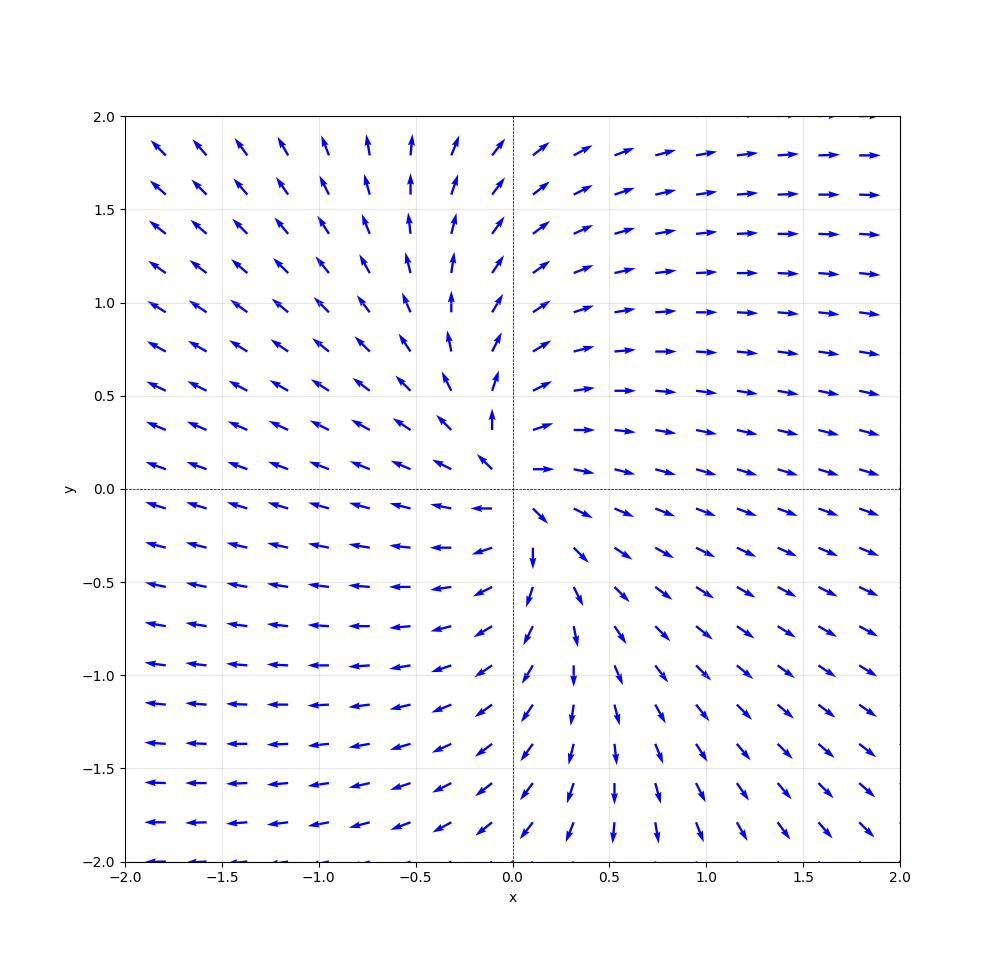
\includegraphics[width=0.8\linewidth]{graph/976.png}
                
        \label{fig:mpr}
        
    \end{figure}

\end{solution}\pagebreak

\section*{Задача 980}
Найти и исследовать особые точки.
$$
    y' = {2x + y}{x - 2y - 5}
$$

\begin{solution}
    $$\begin{cases}
            2x + y = 0 \\
            x - 2y - 5 = 0
        \end{cases} => x = 1, y = -2 $$
    Запишем матрицу 1-го приближения:
    $$ \tilde{A} = \begin{pmatrix}
            1 & -2 \\
            2 & 1
        \end{pmatrix} $$
    $$ |\tilde{A} - \lambda E| = \begin{vmatrix}
            1 - \lambda & -2          \\
            2           & 1 - \lambda
        \end{vmatrix} = (1 - \lambda)^2 + 4 = 0 $$
    $$ \lambda^2 - 2\lambda + 5 = 0 => $$
    $$ => \lambda_{1, 2} = 1 \pm 2 \cdot i => $$
    => фокус.
    \begin{figure}[h]
        \centering
        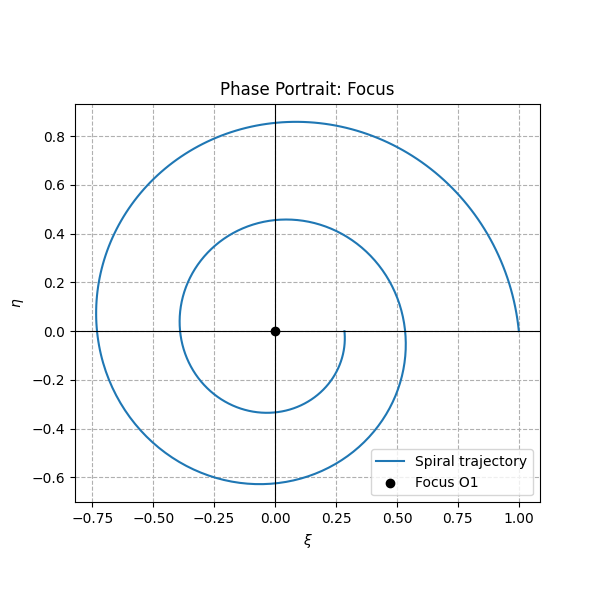
\includegraphics[width=0.8\linewidth]{graph/980.png}
    \end{figure}
\end{solution}
\end{document}
